\subsection{Serie 8}%
\label{sub:serie_8}

\paragraph{Aufgabe 1}%
\label{par:serie_8_aufgabe_1}

Spieler 1 und 2 wechseln sich in einem Spiel mit vollkommener Information darin ab
(beginnend mit Spieler 1), Steine von einem Haufen wegzunehmen.
Zu Beginn des Spiels sind $n > 0$ Steine auf dem Haufen.
Ein Spieler, der am Zug ist, kann einen oder zwei Steine wegnehmen.
Das Spiel endet, wenn kein Stein mehr auf dem Haufen liegt.
Der Spieler, der den letzten Stein wegnimmt, ist der Gewinner.
Die Auszahlung des Gewinners ist 1; die des Verlierers ist 0.
Für $n = 1$ und $n = 2$ gewinnt (in einem teilspielperfekten Gleichgewicht) offenkundig
Spieler 1 dieses Spiel.

\begin{enumerate}
  \item Wer gewinnt für $n = 3$? Wer für $n = 4$?
  \item Können Sie den Gewinner für beliebiges $n$ bestimmen?
\end{enumerate}

\subparagraph{Lösung}%

\begin{enumerate}
  \item Seien \circled{1} bzw. \circled{2} die Aktionen der Spieler. Für $n=3$:
    \begin{center}
      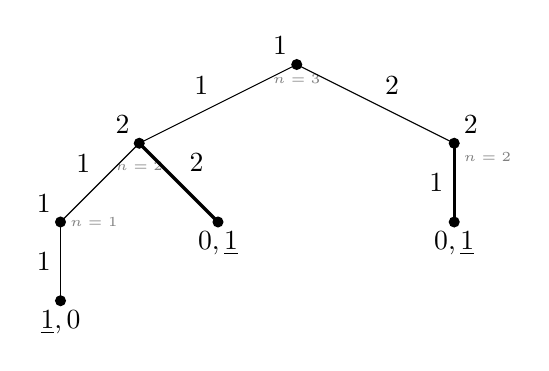
\begin{tikzpicture}
        \fill (0,0) circle (2pt)
          node [above left] {1}
          node [below, gray] {\tiny $n=3$};

        \fill (-2,-1) circle (2pt)
          node [above left] {2}
          node [below, yshift=-3pt, gray] {\tiny $n=2$};
        \fill (2,-1) circle (2pt)
          node [above right] {2}
          node [below right, gray] {\tiny $n=2$};

        \fill (-3,-2) circle (2pt)
          node [above left] {1}
          node [right, gray] {\tiny $n=1$};
        \fill (-1,-2) circle (2pt) node [below] {$0,\underline{1}$};
        \fill (2,-2) circle (2pt) node [below] {$0,\underline{1}$};
        \fill (-3,-3) circle (2pt) node [below] {$\underline{1},0$};

        \draw (0,0) -- (-2,-1) node [midway, above left] {\circled{1}};
        \draw (0,0) -- (2,-1) node [midway, above right] {\circled{2}};
        \draw (-2,-1) -- (-3,-2) node [midway, above left] {\circled{1}};
        \draw [very thick] (-2,-1) -- (-1,-2) node [midway, above right] {\circled{2}};
        \draw [very thick] (2,-1) -- (2,-2) node [midway, left] {\circled{1}};
        \draw (-3,-2) -- (-3,-3) node [midway, left] {\circled{1}};
      \end{tikzpicture}
    \end{center}
    Bei $n=3$ gewinnt immer Spieler 2 bzw. der Spieler,
    der nicht beginnt (der Nachziehende).

    Für $n=4$:
    \begin{center}
      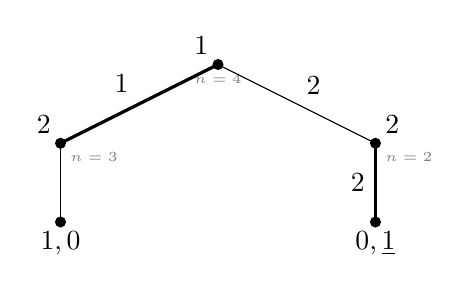
\begin{tikzpicture}
        \fill (0,0) circle (2pt)
          node [above left] {1}
          node [below, gray] {\tiny $n=4$};

        \fill (-2,-1) circle (2pt)
          node [above left] {2}
          node [below right, gray] {\tiny $n=3$};
        \fill (2,-1) circle (2pt)
          node [above right] {2}
          node [below right, gray] {\tiny $n=2$};

        \fill (-2,-2) circle (2pt) node [below] {$1,0$};
        \fill (2,-2) circle (2pt) node [below] {$0,\underline{1}$};

        \draw [very thick] (0,0) -- (-2,-1) node [midway, above left] {\circled{1}};
        \draw (0,0) -- (2,-1) node [midway, above right] {\circled{2}};
        \draw (-2,-1) -- (-2,-2);
        \draw [very thick] (2,-1) -- (2,-2) node [midway, left] {\circled{2}};
      \end{tikzpicture}
    \end{center}
    Bei $n=4$ gewinnt immer Spieler 1 bzw. der Spieler,
    der beginnt (der Anziehende).

  \item Sei $k \in \NaturalNumbers$.
    Für $n$ der Form $3k+1$ bzw. $3k+2$ gewinnt Spieler 1 (der Anziehende),
    indem er einen Stein (bei $3k+1$) bzw. zwei Steine (bei $3k+2$) zieht.
    Für $n$ der Form $3k$ gewinnt Spieler 2 (der Nachziehende).
\end{enumerate}

\paragraph{Aufgabe 2}%
\label{par:serie_8_aufgabe_2}

In einem Spiel mit vollkommener Information gibt es drei Felder: $A, B$ und $C$.
Spieler 1 beginnt das Spiel, indem er auf die Felder positive Geldbeträge
$(x_A, x_B, x_C)$ legt.
Danach ist Spieler 2 am Zug und kann positive Geldbeträge $(y_A, y_B, y_C)$ auf die Felder
legen.
Damit endet das Spiel.
Der Gewinner ist der Spieler, der die meisten Felder gewinnt.
Spieler 1 gewinnt das Feld $f \in \{A,B,C\}$, wenn $x_f > y_f$ gilt;
ansonsten gewinnt Spieler 2 das Feld.
Gewinnt Spieler $i$, erhält er einen Preis in Höhe von $V_i > 0$.
Jeder Spieler muss die Summe seiner Gebote bezahlen.
Wenn Spieler 1 gewinnt, ist seine Auszahlung also
\begin{align*}
  V_1 - x_A - x_B - x_C,
\end{align*}
wenn er verliert, ist sie
\begin{align*}
  - x_A - x_B - x_C.
\end{align*}
Die Auszahlungen von Spieler 2 sind entsprechend.

\begin{enumerate}
  \item Bestimmen Sie das (jeweils eindeutig bestimmte) Ergebnis der teilspielperfekten
    Gleichgewichte für den Fall $V_1 = V_2 = 300$.
    (Hinweis: eine vollständige Bestimmung der Gleichgewichtsstrategien ist hierfür nicht
    erforderlich; Sie dürfen in der Bearbeitung unterstellen, dass es teilspielperfekte
    Gleichgewichte gibt.)
  \item Wiederholen Sie die Aufgabe für den Fall $V_1 = 300, V_2 = 100$.
\end{enumerate}

\subparagraph{Lösung}%
\begin{enumerate}
  \item Angenommen Spieler 1 setzt die Beträge $(x_A, x_B, x_C)$.
    Sei o.\,B.\,d.\,A. $x_A \leq x_B \leq x_C$.
    Wenn $x_A + x_B \leq 300$ gilt, dann setzt Spieler 2 die Beträge
    $(y_A, y_B, 0) = (x_A, x_B, 0)$, ansonsten setzt er die Beträge $(0,0,0)$.
    Die beste Antwort auf die Strategie von Spieler 1 ist $(0,0,0)$ zu setzen.

  \item Angenommen Spieler 1 setzt die Beträge $(x_A, x_B, x_C)$.
    Sei o.\,B.\,d.\,A. $x_A \leq x_B \leq x_C$.
    Wenn $x_A + x_B \leq 100$ gilt, dann setzt Spieler 2 die Beträge
    $(y_A, y_B, 0) = (x_A, x_B, 0)$, ansonsten setzt er die Beträge $(0,0,0)$.
    Spieler 1 muss daher die Beträge so wählen, dass die Summe der beiden kleinsten
    Beträge echt größer als $100$ ist,
    also z.\,B. $(50,50,51)$ oder mit $ε > 0$: $(50,50,50+ε)$, je nachdem was erlaubt ist.
\end{enumerate}

\paragraph{Aufgabe 3}%
\label{par:serie_8_aufgabe_3}

Betrachten Sie das folgende Verhandlungsspiel.
In Runde 1 macht Spieler 1 ein Angebot $x \in [0, 1]$; daraufhin entscheidet Spieler 2, ob
er das Angebot annimmt oder ablehnt.
Wenn er ablehnt, dann beginnt Runde 2 und Spieler 2 macht ein Angebot, welches Spieler 1
entweder annimmt oder ablehnt.
Einigen sich die Spieler in Runde $t$ auf ein Angebot $x_t$, erhalten sie die Payoffs
\begin{align*}
  (\alpha^t x_t, \beta^t (1-x_t)) \text{ mit $\alpha, \beta \in (0,1)$.}
\end{align*}
Das Spiel endet in Periode $T=3$, wenn das Angebot nicht angenommen wird, mit einer
Auszahlung von $(0,0)$.

\begin{enumerate}
  \item Bestimmen Sie das SPNE.
  \item Welche Auszahlungen erhalten die Spieler?
  \item Berechnen Sie die Auszahlungen für
    $(\alpha, \beta) = (0.8, 0.9)$ und
    $(\alpha, \beta) = (0.9, 0.8)$.
\end{enumerate}

\subparagraph{Lösung}%

\begin{enumerate}
  \item Seien $a$ für \emph{akzeptieren}
    und $z$ für \emph{zurückweisen} die Aktionen der Spieler.
    Der Spielbaum hat folgende Gestalt:
    \begin{center}
      \begin{tikzpicture}
        \fill [gray!25] (0,0) -- (-1.5,-1) -- (1.5,-1) -- cycle;
        \fill (0,0) circle (2pt) node [above] {1};
        \fill (-1,-1) circle (2pt) node [above left] {2};
        \fill (-1.5,-2) circle (2pt) node [below] {$α x_1, β(1-x_1)$};
        \draw (0,0) -- (-1,-1);
        \draw (-1,-1) -- (-1.5,-2) node [midway, above left] {$a$};
        \draw (-1,-1) -- (1.5,-2) node [midway, above right] {$z$};

        \fill [gray!25] (1.5,-2) -- (0,-3) -- (3,-3) -- cycle;
        \fill (1.5,-2) circle (2pt) node [above] {2};
        \fill (2,-3) circle (2pt) node [above right] {1};
        \fill (0,-4) circle (2pt) node [below] {$α^2 x_2, β^2(1-x_2)$};
        \draw (1.5,-2) -- (2,-3);
        \draw (2,-3) -- (0,-4) node [midway, above left] {$a$};
        \draw (2,-3) -- (3,-4) node [midway, above right] {$z$};

        \fill [gray!25] (3,-4) -- (1.5,-5) -- (4.5,-5) -- cycle;
        \fill (3,-4) circle (2pt) node [above] {1};
        \fill (3.75,-5) circle (2pt) node [above right] {2};
        \fill (1.5,-6) circle (2pt) node [below] {$α^3 x_3, β^3(1-x_3)$};
        \fill (4.5,-6) circle (2pt) node [below] {$0,0$};
        \draw (3,-4) -- (3.75, -5);
        \draw (3.75,-5) -- (1.5,-6) node [midway, above left] {$a$};
        \draw (3.75,-5) -- (4.5,-6) node [midway, above right] {$z$};
      \end{tikzpicture}
    \end{center}

    Wir betrachten das Teilspiel der letzten Runde (Runde 3):
    \begin{center}
      \begin{tikzpicture}
        \fill [gray!25] (3,-4) -- (1.5,-5) -- (4.5,-5) -- cycle;
        \fill (3,-4) circle (2pt) node [above] {1};
        \fill (3.75,-5) circle (2pt) node [above right] {2};
        \fill (1.5,-6) circle (2pt) node [below] {$α^3 x_3, β^3(1-x_3)$};
        \fill (4.5,-6) circle (2pt) node [below] {$0,0$};
        \draw (3,-4) -- (3.75, -5);
        \draw (3.75,-5) -- (1.5,-6) node [midway, above left] {$a$};
        \draw (3.75,-5) -- (4.5,-6) node [midway, above right] {$z$};
      \end{tikzpicture}
    \end{center}
    Das Ultimatumspiel lehrt uns: Spieler 2 akzeptiert $\iff x_3 \leq 1$.
    Damit macht Spieler 1 das Angebot $x_3 = 1$, Spieler 2 akzeptiert und die Spieler erhalten
    folgende Auszahlungen:
    \begin{align*}
      u_1 & = α^3 \cdot 1 = α^3\\
      u_2 & = β^3 \cdot 0 = 0
    \end{align*}
    Im Teilspiel der vorletzten Runde (Runde 2) gilt:
    \begin{center}
      \begin{tikzpicture}
        \fill [gray!25] (1.5,-2) -- (0,-3) -- (3,-3) -- cycle;
        \fill (1.5,-2) circle (2pt) node [above] {2};
        \fill (2,-3) circle (2pt) node [above right] {1};
        \fill (0,-4) circle (2pt) node [below] {$α^2 x_2, β^2(1-x_2)$};
        \fill (3,-4) circle (2pt) node [below] {$α^3, 0$};
        \draw (1.5,-2) -- (2,-3);
        \draw (2,-3) -- (0,-4) node [midway, above left] {$a$};
        \draw (2,-3) -- (3,-4) node [midway, above right] {$z$};
      \end{tikzpicture}
    \end{center}
    Spieler 1 akzeptiert $\iff α^2 x_2 \geq α^3$,
    daher bietet Spieler 2 $x_2 = α$ an,
    Spieler 1 akzeptiert und die Auszahlungen der Spieler betragen:
    \begin{align*}
      u_1 & = α^3\\
      u_2 & = β^2(1-α)
    \end{align*}
    In der ersten Runde ergibt sich folgende Situation:
    \begin{center}
      \begin{tikzpicture}
        \fill [gray!25] (0,0) -- (-1.5,-1) -- (1.5,-1) -- cycle;
        \fill (0,0) circle (2pt) node [above] {1};
        \fill (-1,-1) circle (2pt) node [above left] {2};
        \fill (-1.5,-2) circle (2pt) node [below] {$α x_1, β(1-x_1)$};
        \fill (1.5,-2) circle (2pt) node [below] {$α^3, β^2(1-α)$};
        \draw (0,0) -- (-1,-1);
        \draw (-1,-1) -- (-1.5,-2) node [midway, above left] {$a$};
        \draw (-1,-1) -- (1.5,-2) node [midway, above right] {$z$};
      \end{tikzpicture}
    \end{center}
    Spieler 2 akzeptiert $\iff β(1-x_1) \geq β^2(1-α) \iff 1-β(1-α) \geq x_1$.
    Spieler 1 will die Auszahlung maximieren,
    also bietet er $x_1 = 1-β(1-α)$ an und Spieler 2 akzeptiert.
    Damit gilt für das SPNE: Spieler 1 bietet $x_1 = 1-β(1-α)$ und Spieler 2 akzeptiert.

  \item Die Auszahlungen betragen:
    \begin{align*}
      u_1 & = α(1-β(1-α))\\
      u_2 & = β(1-(1-β(1-α))) = β^2 (1-α)
    \end{align*}

  \item Für $(α, β) = (0.8, 0.9)$ ergibt sich:
    \begin{align*}
      u_1 & = α(1-β(1-α)) = 0.656\\
      u_2 & = β^2 (1-α) = 0.162
    \end{align*}
  Für $(α, β) = (0.9, 0.8)$ ergibt sich:
    \begin{align*}
      u_1 & = α(1-β(1-α)) = 0.828\\
      u_2 & = β^2 (1-α) = 0.064
    \end{align*}

  Bonusfrage: für welche Werte von $α$ und $β$ erhält Spieler 2 eine höhere Auszahlung als
  Spieler 1?
  \href{https://www.wolframalpha.com/input/?i=a%281-b%281-a%29%29+%3C+b%5E2%281-a%29+and+0%3Ca%3C1+and+0%3Cb%3C1}{WolframAlpha}
  liefert folgendes Ergebnis:
  \begin{align*}
    0 < α < \frac{\sqrt{5} - 1}{2} = φ - 1 \approx 0.618
    \quad
    \text{und}
    \quad
    \frac{1}{2} \left( \sqrt{\frac{α \left( α^2-α-4 \right)}{α-1}} - α \right) < β < 1
  \end{align*}
  wobei $φ$ der goldene Schnitt ist.
\end{enumerate}

\paragraph{Aufgabe 4}%
\label{par:serie_8_aufgabe_4}

Betrachten Sie folgendes \emph{Game of Chicken}:
\begin{center}
  \begin{tabular}{ccc}
    & \emph{Dove} & \emph{Hawk}\\
    \cmidrule{2-3}
    \emph{Dove} & $2,2$ & $0,3$\\
    \cmidrule{2-3}
    \emph{Hawk} & $3,0$ & $-1,-1$\\
    \cmidrule{2-3}
  \end{tabular}
\end{center}
Nehmen Sie an, die zwei Spieler 1 und 2 wiederholen dieses Spiel nacheinander 100 Mal.
Die Auszahlung des Spielers $i \in \{1,2\}$ im wiederholten Spiel sei dabei einfach die
Summe der in jedem Stufenspiel durch diesen Spieler erzielten Nutzenwerte.
Betrachten Sie folgende dynamische Strategie $s$:
\begin{itemize}
  \item Wenn $t < 100$ und der Gegenspieler in der Vergangenheit bis einschließlich $t-1$
    immer \emph{Dove} wählte: wähle \emph{Dove}.
  \item Wenn $t = 100$ und der Gegenspieler in der Vergangenheit bis einschließlich $t-1$
    immer \emph{Dove} wählte: spiele die gemischte Strategie
    $\left( \frac{1}{2}, \frac{1}{2} \right)$.
  \item Wenn irgendeiner der Spieler in irgendeiner Stufe $t < 100$ nicht \emph{Dove}
    wählt: schaue auf die Stufe $\tilde{t}$, in der die Abweichung erstmalig auftritt und
    spiele für den Rest des Spiels diejenige Strategie, die in Stufe $\tilde{t}$
    \textbf{nicht} gewählt wurde.
\end{itemize}

\begin{enumerate}
  \item Weshalb ist $(s,s)$ ein Nash-Gleichgewicht?
  \item Zeigen Sie, dass $(s,s)$ teilspielperfekt ist.
  \item Welche Eigenschaft des \emph{Chicken-Games} macht es möglich, dass ein Resultat in
    Analogie zu den \emph{Folk}-Theoremen auch im Fall eines endlich oft wiederholten
    Spiels auftritt?
\end{enumerate}
